\documentclass{article}
\usepackage{fullpage,graphicx}
\usepackage{amsmath,amsfonts,amsthm,amssymb,multirow}
\usepackage{algorithmic,url}
\usepackage{tikz}
\usetikzlibrary{decorations.pathreplacing, shapes,positioning}
\usepackage[ruled,vlined,commentsnumbered,titlenotnumbered]{algorithm2e}
\newcommand{\expecting}[1]{\noindent{[\textbf{We are expecting:} \em #1\em]}}
\newcommand{\hint}[1]{\noindent{[\textbf{HINT:} \em #1\em]}}
\newcommand{\pts}[1]{\textbf{(#1 pt.)}}


\begin{document}
\noindent
CS 161 \hfill \textbf{Problem Set 6} \newline 
{Winter 2019} \hfill \textbf{Due:} Friday, March 8, 2019, at 3pm on Gradescope

\noindent
\rule{\linewidth}{0.4pt}
\noindent
\section*{Exercise}
Please do the exercises on your own.

\noindent
\rule{\linewidth}{0.4pt}
\begin{enumerate}

\item\pts{8} Let $A$ be an array of length $n$ containing real numbers.  A \em longest increasing subsequence \em (LIS) of $A$ is a sequence $0 \leq i_0 < i_1 < \ldots i_\ell < n$ so that $A[i_0] < A[i_1] < \cdots < A[i_\ell]$, so that $\ell$ is as large as possible.  For example, if 
$A = [6,3,2,5,6,4,8]$, then a LIS is $i_0 = 1, i_1 = 3, i_2 = 4, i_3 = 6$ corresponding to the subsequence $3,5,6,8$.  (Notice that a longest increasing subsequence doesn't need to be unique).

In the following parts, we'll walk through the recipe that we saw in class for coming up with DP algorithms to develop an $O(n^2)$-time algorithm for finding an LIS. 
\begin{enumerate}
\item\pts{2} \textbf{(Identify optimal sub-structure and a recursive relationship).}  We'll come up with the sub-problems and recursive relationship for you, although you will have to justify it.  Let $D[i]$ be the length of the longest increasing subsequence of $[A[0], \ldots, A[i]]$ that ends on $A[i]$.
Explain why
\[ D[i] = \max\left(\{ D[k] + 1\,:\, 0 \leq k < i, A[k] < A[i] \} \cup \{1\} \right). \]

\expecting{A short informal explanation (a paragraph or so).  It might be good practice to write a formal proof, but this is not required for credit.}

\item\pts{3} \textbf{(Develop a DP algorithm to find the value of the optimal solution)} Use the relationship about to design a dynamic programming algorithm returns the \em length \em of the longest increasing subsequence.  Your algorithm should run in time $O(n^2)$ and should fill in the array $D$ defined above.

\expecting{Pseudocode.  No justification is required.}

\item \pts{3} \textbf{(Adapt your DP algorithm to return the optimal solution)} Adapt your algorithm above to return an actual LIS instead of its length.  Your algorithm should run in time $O(n^2)$.

\expecting{Pseudocode \textbf{AND} a short English explanation of what your algorithm is doing.  You do not need to justify that it is correct.}

\end{enumerate}

\textbf{Note:} Actually, there is an $O(n\log(n))$-time algorithm to find an LIS, which is faster than the DP solution in this exercise!  


\end{enumerate}
\newpage
\noindent
\rule{\linewidth}{0.4pt}
\section*{Problems}

You may talk with your fellow CS161-ers about the problems.  However:
\begin{itemize}
	\item Try the problems on your own \em before \em collaborating.
	\item Write up your answers yourself, in your own words.   You should never share your typed-up solutions with your collaborators.
	\item If you collaborated, list the names of the students you collaborated with at the beginning of each problem.
\end{itemize}

\noindent
\rule{\linewidth}{0.4pt}


\begin{enumerate}
\setcounter{enumi}{1}

\item \pts{7} \textbf{[MinElementSum.]}
Consider the following problem, \textsc{MinElementSum}.
\begin{quote}
\textsc{MinElementSum}$(n,S)$:
Let $S$ be a set of positive integers, and let $n$ be a non-negative integer.  Find the minimal number of elements of $S$ needed to write $n$ as a sum of elements of $S$ (possibly with repetitions).  If there is no way to write $n$ as a sum of elements of $S$, return \texttt{None}.
\end{quote}

For example, if $S = \{1,4,7\}$ and $n = 10$, then we can write $n = 1 + 1 + 1 + 7$ and that uses four elements of $S$.  The solution to the problem would be ``4."   On the other hand if $S = \{4,7\}$ and $n=10$, then the solution to the problem would be ``\texttt{None},'' because there is no way to make $10$ out of $4$ and $7$.

Your friend has devised a divide-and-conquer algorithm to solve \textsc{MinElementSum}.  Their pseudocode is below.
\begin{verbatim}
def minElementSum(n, S):
     if n == 0:
         return 0
     if n < min(S):
         return None
     candidates = []
     for s in S:
         cand = minElementSum( n-s, S )
         if cand is not None: 
              candidates.append( cand + 1 )
     if len(candidates) == 0:
         return None
     return min(candidates) 
\end{verbatim}

Your friend's algorithm correctly solves \textsc{MinElementSum}.  Before you start doing the problems on the next page, it would be a good idea to walk through the algorithm and to understand what this algorithm is doing and why it works.  

\vfill \hfill [Questions on next page]
\newpage

\begin{enumerate}
\item \pts{1} Argue that for $S = \{1,2\}$, your friend's algorithm has exponential running time.  (That is, running time of the form $2^{\Omega(n)}$).  
You may use any statement that we have seen in class.  

\hint{Consider the example of the Fibonacci numbers that we saw in class.}

\expecting{
\begin{itemize}
\item A recurrence relation that the running time of your friend's algorithm satisfies when $S = \{1,2\}$.
\item A convincing argument that the closed form for this expression is $2^{\Omega(n)}$.  You do not need to write a formal proof.  \end{itemize}}

\item \pts{3} Turn your friend's algorithm into a top-down dynamic programming algorithm.  
Your algorithm should take time $O(n|S|)$.

\hint{Add an array to the pseudocode above to prevent it from solving the same sub-problem repeatedly.}


\expecting{\begin{itemize} 
\item Pseudocode \textbf{AND} a short English description of the idea of your algorithm.
\item An informal justification of the running time.\end{itemize}}


\item \pts{3} Turn your friend's algorithm into a bottom-up dynamic programming algorithm.  
Your algorithm should take time $O(n|S|)$.

\hint{Fill in the array you used in part (b) iteratively, from the bottom up.}

\expecting{\begin{itemize} 
\item Pseudocode \textbf{AND} a short English description of the idea of your algorithm.
\item An informal justification of the running time.\end{itemize}}
\end{enumerate}

\newpage
\item \pts{6} \textbf{[Rotten Tomatoes.]}
You are planting tomato plants in a garden, and the garden has $n$ spots arranged in a line.  Different spots in the garden will result in different quality tomatoes: suppose that the location $i$ will result in tomatoes of deliciousness $T[i]$, where $T[i]$ is a positive integer.  Further, you cannot plant two plants directly next to each other, because they will compete for resources and wilt.  
Your goal is to create the most deliciousness possible (summed up over all of the tomato plants).  

\textbf{For example,} if the input was
$ T = [21,4,6,20,2,5],$
then you should plant tomatoes in the pattern
\begin{center}
    \begin{tikzpicture}
\foreach \i in {1,2,3,4,5,6}
{
\draw (\i -1, 0) rectangle (\i, 1);
}
\foreach \i in {1,4,6}
{
\node at (\i -.5, .5) {\includegraphics[width=.8cm]{th.jpeg}};
}
\end{tikzpicture}
\end{center}
and you would obtain deliciousness $21 +20+5 = 46$.  You would \textbf{not} be allowed to plant tomatoes in the pattern
\begin{center}
\begin{tikzpicture}
\foreach \i in {1,2,3,4,5,6}
{
\draw (\i -1, 0) rectangle (\i, 1);
}
\foreach \i in {1,2,4,6}
{
\node at (\i -.5, .5) {\includegraphics[width=.8cm]{th.jpeg}};
}
\end{tikzpicture}
\end{center}
because there are two tomato plants next to each other. 

In this question, you will
design a dynamic programming algorithm which runs in time $O(n)$ which takes as input the array $T$ and returns the maximum deliciousness possible given $T$.  Do this by answering the two parts below.

\begin{enumerate}
	\item \pts{3} What sub-problems will you use in your dynamic programming algorithm?  What is the recursive relationship which is satisfied between the sub-problems? What is the base case for this recursive relationship? 

\expecting{\begin{itemize}
\item A clear description of your sub-problems.
\item A recursive relationship that they satisfy, along with a base case.
\item An informal justification that the recursive relationship is correct.
\end{itemize}}
	
	
	\item \pts{3} Write pseudocode for your algorithm.  Your algorithm should take as input the array $T$, and return a single number which is the maximum amount of deliciousness possible.  Your algorithm does not need to output the optimal way to plant the tomatoes.

\expecting{Pseudocode \textbf{AND} a clear English description.  You do not need to justify that your algorithm is correct, but correctness should follow from your reasoning in part (a).}
\end{enumerate}



\newpage
\item \pts{6} \textbf{[Fish fish eat eat fish.] }
Plucky the Pedantic Penguin enjoys fish, and he has discovered that on some days the fish supply is better in Lake A and some days the fish supply is better in Lake B.
He has access to two tables $A$ and $B$, where $A[i]$ is the number of fish he can catch in Lake A on day $i$, and $B[i]$ is the number of fish he can catch in Lake B on day $i$, for $i=0,\ldots,n-1$.    

If Plucky is at Lake $A$ on day $i$ and wants to be at Lake $B$ on day $i+1$, he may pay $L$ fish to a polar bear who can take him from Lake $A$ to Lake $B$ overnight; the same is true if he wants to go from Lake $B$ back to Lake $A$. 
The polar bear does not accept credit, so \textbf{Plucky  must pay \em before \em he travels}. (And if he cannot pay, he cannot travel).

Assume that when day $0$ begins, Plucky is at Lake $A$, and he has zero fish.  Also assume that $A[i]$ and $B[i]$ are positive integers for $i =0,\ldots,n-1$ and that $L$ is also a positive integer. 


\fbox{
\begin{minipage}{0.9\textwidth}
For example, suppose that $n=3$, $L=3$, and that $A$ and $B$ are given by
$A = [5,2,3]$ and  $B = [2,7,4].$
Then Plucky might do:
\begin{center}
\begin{tikzpicture}
\node at (1, .6) {Lake $A$};
\node at (7, .6) {Lake $B$};
\begin{scope}[yscale=.8]
\draw [decorate,decoration={brace,amplitude=10pt},xshift=-4pt,yshift=0pt]
(0,-2.4) -- (0,.4)node [black,midway,xshift=-30pt] {Day 0};
\node(p0) at (1,0) {\includegraphics[width=.5cm]{plucky}};
\node(p1) at (1,-2) {\includegraphics[width=.5cm]{plucky}};
\node at (1.7, 0) {$0$ fish};
\node at (1.7, -1.7) {$5$ fish};
\draw[dashed] (p0) to node[right,pos=0.5] {$+5$} (p1);
\end{scope}
\begin{scope}[yscale=.8,yshift=-3cm]
\draw [decorate,decoration={brace,amplitude=10pt},xshift=-4pt,yshift=0pt]
(0,-2.4) -- (0,.4)node [black,midway,xshift=-30pt] {Day 1};
\node(p2) at (7,0) {\includegraphics[width=.5cm]{plucky}};
\node(p3) at (7,-2) {\includegraphics[width=.5cm]{plucky}};
\node at (7.7, 0) {$2$ fish};
\node at (7.7, -2) {$9$ fish};
\draw[dashed] (p2) to node[right,pos=0.5] {$+7$} (p3);
\end{scope}
\begin{scope}[yscale=0.8, yshift=-6cm]
\draw [decorate,decoration={brace,amplitude=10pt},xshift=-4pt,yshift=0pt]
(0,-2.4) -- (0,.4)node [black,midway,xshift=-30pt] {Day 2};
\node(p4) at (7,0) {\includegraphics[width=.5cm]{plucky}};
\node(p5) at (7,-2) {\includegraphics[width=.5cm]{plucky}};
\node at (7.7, 0) {$9$ fish};
\node at (7.7, -2) {$13$ fish};
\draw[dashed] (p4) to node[right,pos=0.5] {$+4$} (p5);
\end{scope}
\draw[dashed] (p1) to node[above,pos=0.5] {$-3$} (p2);
\end{tikzpicture}
\end{center}

So Plucky's total fish at the end of day $n-1=2$ is $13$.
\end{minipage}
}

In this question, you will design an $O(n)$-time dynamic programming algorithm that finds the maximum number of fish that Plucky can have at the end of day $n-1$.   Do this by answering the two parts below.


\begin{enumerate}
	\item \pts{3} What sub-problems will you use in your dynamic programming algorithm?  What is the recursive relationship which is satisfied between the sub-problems?  What is the base case for this recursive relationship? 

\expecting{\begin{itemize}
\item A clear description of your sub-problems.
\item A recursive relationship that they satisfy, along with a base case.
\item An informal justification that the recursive relationship is correct.
\end{itemize}}

	
	\item \pts{3} Design a dynamic programming algorithm that takes as input $A,B,L$ and $n$, and in time $O(n)$ returns the maximum number of fish that Plucky can have at the end of day $n-1$.

\expecting{Pseudocode \textbf{AND} a short English description of what it does and why it works, and a justification of why it runs in time $O(n)$.}
\end{enumerate}



\newpage
\textbf{This problem set is long enough}, but more practice with dynamic programming is always good.  If you'd like another practice problem (or just miss Socrates the Scientific Squirrel), you can do the problem below for one bonus point.  To get the bonus point, you should complete the whole problem.
\item \pts{NOT REQUIRED, WORTH 1 BONUS} \textbf{[Nuts! (part 2)]}

\begin{minipage}{.5\textwidth}
Socrates the Scientific Squirrel (from HW1) is back!
Recall that Socrates lives in a very tall tree with $n$ branches, and she wants to find out what is the lowest branch $i \in \{1, \ldots, n\}$ so that an acorn will break open when dropped from branch $i$.  If an acorn breaks open when dropped from branch $i$, then an acorn will also break open when dropped from branch $j$ for any $j \geq i$.  
(If no branch will break an acorn, Socrates should return $n+1$).
\newline \newline
The catch is that, once an acorn is broken open, Socrates will eat it immediately and it can't be dropped again.
\newline\newline
In HW1, you designed a strategy for Socrates to use very few drops, given that she had $k$ acorns.  She was pretty pleased with that algorithm, but now she wants to compute \em exactly \em the number of drops she needs, in the worst case.
\end{minipage}
\hspace{.5cm}
\begin{minipage}{.4\textwidth}
\hfill
\begin{tikzpicture}
\node{
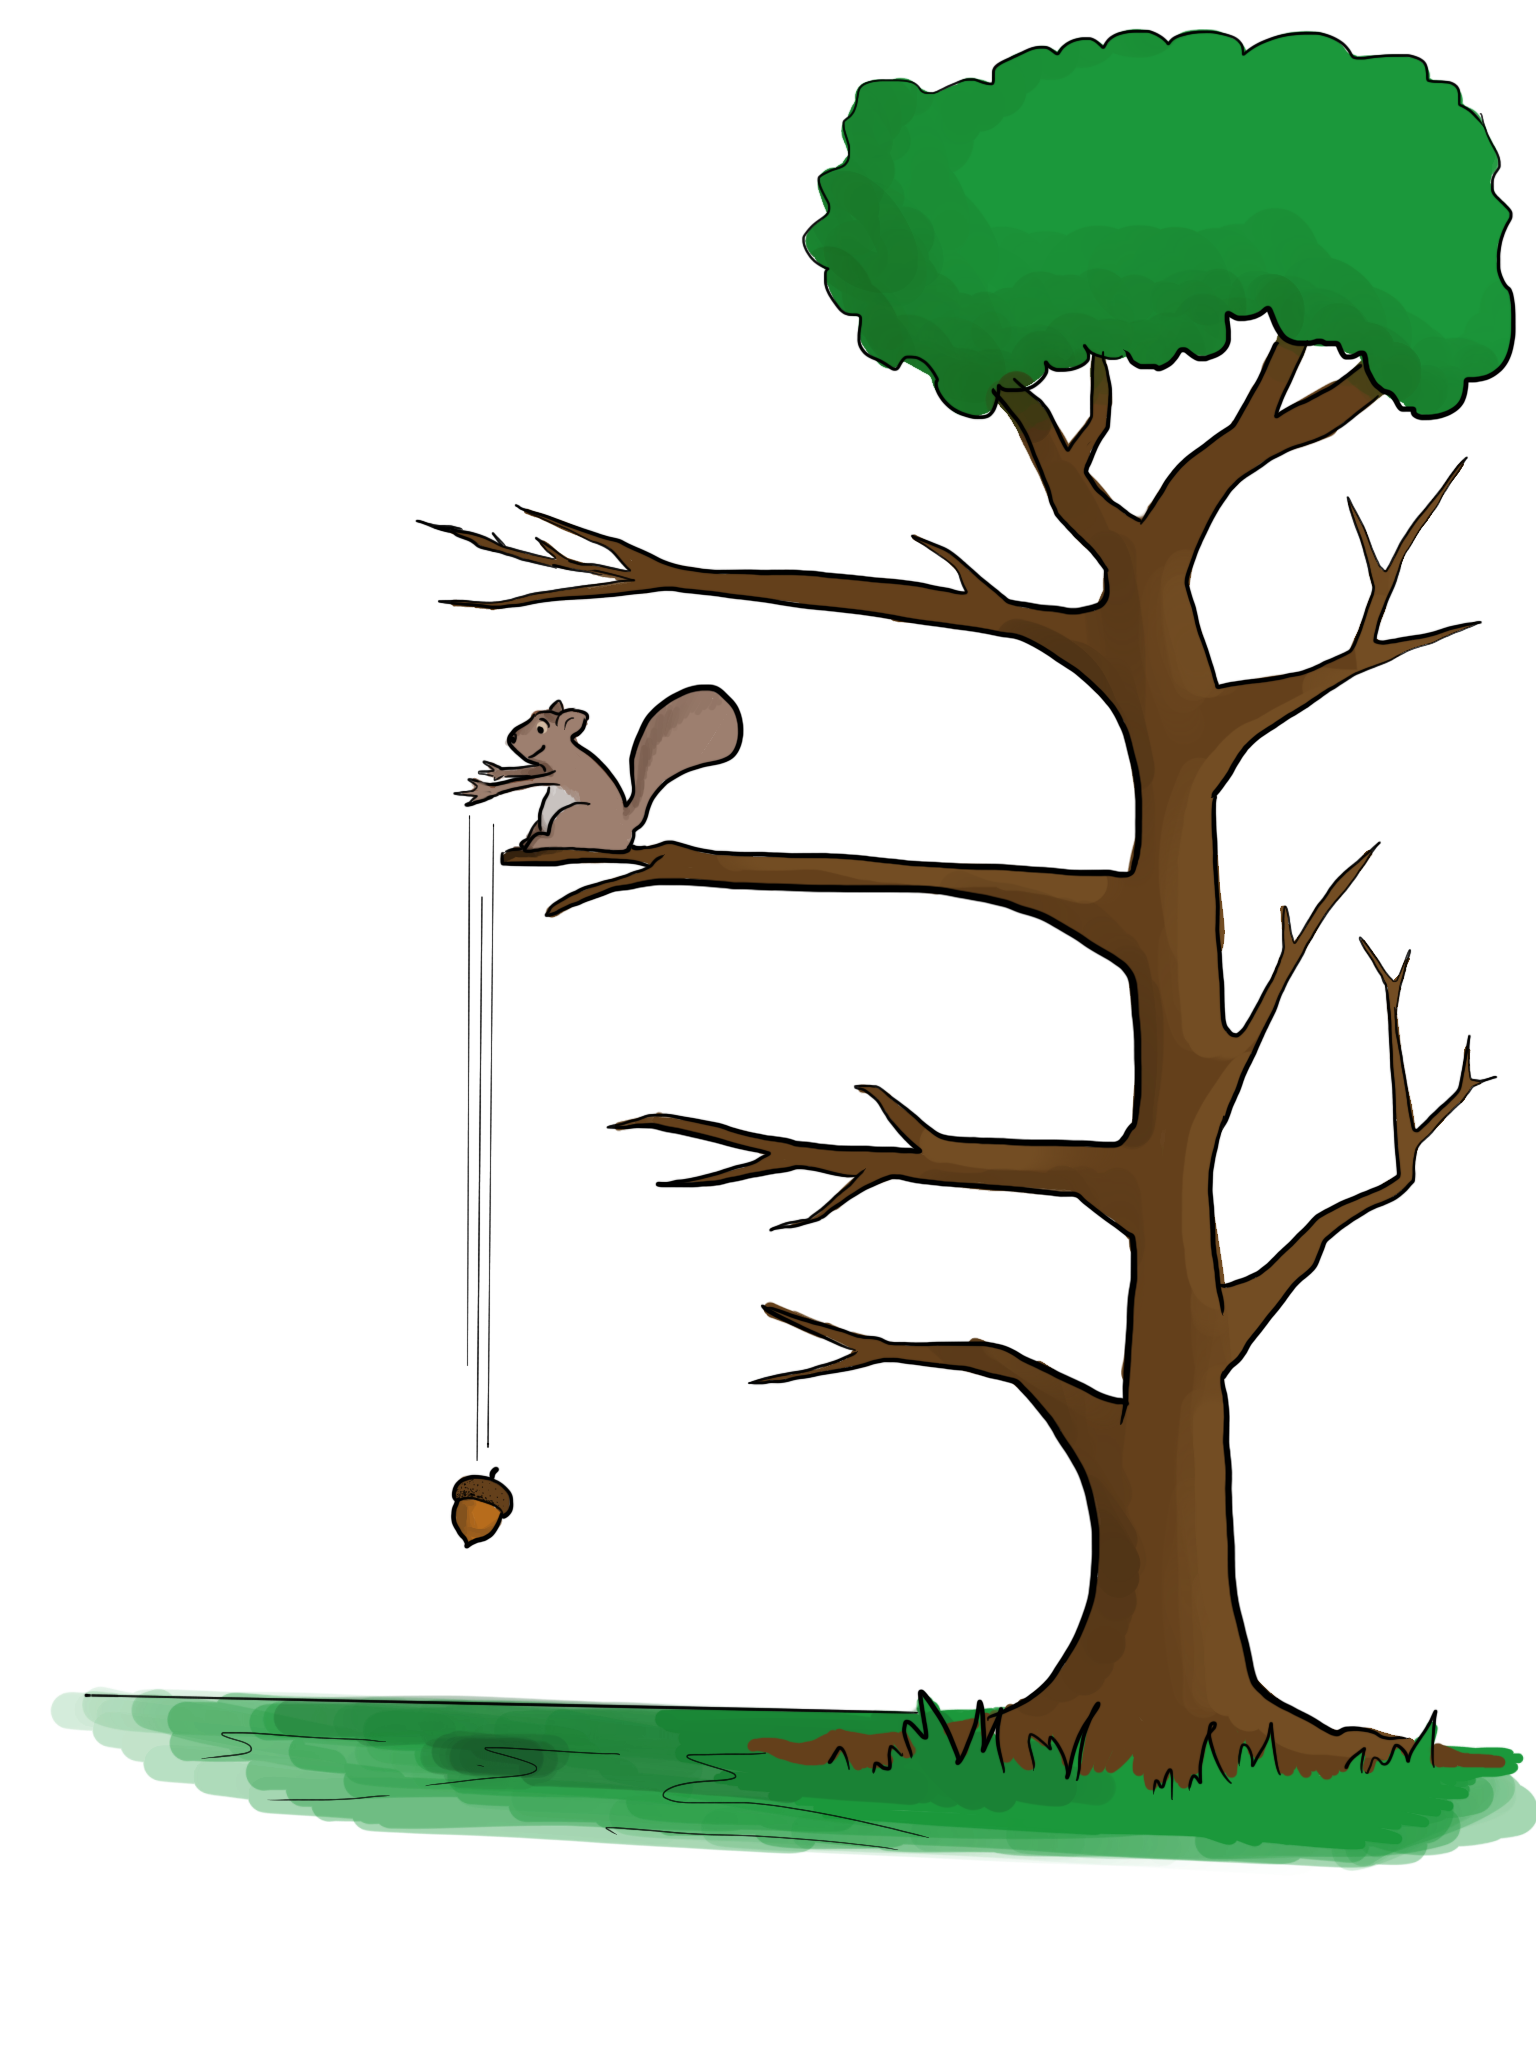
\includegraphics[width=6cm]{squirrel}};
\node(bn) at (-2.5,1.8) {Branch $n$};
\node(b0) at (-2.2,-1.25) {Branch $1$};
\node(b1) at (-2.2,-.55) {Branch $2$};
\draw(b0) -- (-.3, -1.25);
\draw(b1) -- (-.7, -.55);
\end{tikzpicture}
\end{minipage}

\vspace{.5cm}
For $n \geq 0$ and $k \geq 1$, let $D[n,k]$ be the \em optimal worst-case number of drops \em that Socrates needs to determine the correct branch out of $n$ branches using $k$ acorns.    That is, $D[n,k]$ is the number of drops that the best algorithm would use in the worst-case.
\begin{enumerate}
\item For any $1 \leq j \leq k$, what is $D[0,j]$? What is $D[1,j]$?  For any $1 \leq m \leq n$, what is $D[m,1]$? 
(Note that if $n=0$, then Socrates needs zero drops to identify the correct branch, since there are no branches).

\expecting{Your answer.  No justification required.}

\item Suppose the best algorithm drops the first acorn from branch $x \in \{1, \ldots, n\}$. Write a formula for the optimal worst-case number of drops remaining in terms of $D[x-1,k-1]$ and $D[n-x,k]$.  

\expecting{Your formula and an informal explanation of why this formula is correct.}

\item  Write a formula for $D[n,k]$ in terms of values $D[m,j]$ for $j \leq k$ and $m < n$.  

\hint{Use part (b).}

\expecting{Your formula and an informal explanation of why this formula is correct.}

\item Design a dynamic programming algorithm which will compute $D[n,k]$ in time $O(n^2k)$. 

\hint{Use parts (a) and (c).}

\expecting{Pseudocode \text{AND} an English description of how it works, as well as an informal justification of the running time.  You do not need to justify that it is correct.}
\end{enumerate}


\end{enumerate}
\end{document}
